% interactnlmsample.tex
% v1.05 - August 2017

\documentclass[]{interact}

\usepackage{epstopdf}% To incorporate .eps illustrations using PDFLaTeX, etc.
\usepackage[caption=false]{subfig}% Support for small, `sub' figures and tables
%\usepackage[nolists,tablesfirst]{endfloat}% To `separate' figures and tables from text if required
%\usepackage[doublespacing]{setspace}% To produce a `double spaced' document if required
%\setlength\parindent{24pt}% To increase paragraph indentation when line spacing is doubled

\usepackage[numbers,sort&compress]{natbib}% Citation support using natbib.sty
\bibpunct[, ]{[}{]}{,}{n}{,}{,}% Citation support using natbib.sty
\renewcommand\bibfont{\fontsize{10}{12}\selectfont}% Bibliography support using natbib.sty
\makeatletter% @ becomes a letter
\def\NAT@def@citea{\def\@citea{\NAT@separator}}% Suppress spaces between citations using natbib.sty
\makeatother% @ becomes a symbol again

\theoremstyle{plain}% Theorem-like structures provided by amsthm.sty
\newtheorem{theorem}{Theorem}[section]
\newtheorem{lemma}[theorem]{Lemma}
\newtheorem{corollary}[theorem]{Corollary}
\newtheorem{proposition}[theorem]{Proposition}

\theoremstyle{definition}
\newtheorem{definition}[theorem]{Definition}
\newtheorem{example}[theorem]{Example}

\theoremstyle{remark}
\newtheorem{remark}{Remark}
\newtheorem{notation}{Notation}

\begin{document}

% \articletype{ARTICLE TEMPLATE}% Specify the article type or omit as appropriate

\title{aaa}

\author{
\name{Yuya Okada\textsuperscript{a}\thanks{CONTACT Yuya~Okada. Email: okada@hfg.sc.e.titech.ac.jp}, Hiroki Sugawara\textsuperscript{b}, 
    Hiroaki Soya\textsuperscript{b}, Takeshi Hatanaka\textsuperscript{a}}
\affil{\textsuperscript{a}Tokyo Institute of Technology, Tokyo, Japan}
\affil{\textsuperscript{b}Yokogawa Electric Corporation, Tokyo, Japan}
}

\maketitle

\begin{abstract}

\end{abstract}

\begin{keywords}
% Sections; lists; figures; tables; mathematics; fonts; references; appendices
\end{keywords}


\section{Introduction}

\section{Problem Statement}
% Let us consider there are $M$ types heterogeneous robots, of which $r_m,~m\in\{1,...,M\}$ has $N_m$ robots each.
% In this section, when assigning tasks to robots, we use performed tasks, the robots, times and targets where tasks reside as indices.
% Let us consider M types heterogeneous robots and the number $N_m$ of robot $m\in\{1,2,...M\}$ among them.
% Where the set of robots $m$ is $\mathcal{R}_m=\{r^m_1,r^m_2,...,r^m_{N_m}\}$ and the set of all robots are $\mathcal{R}=\mathcal{R}_1\cup\mathcal{R}_2\cup ... \cup\mathcal{R}_M$.
% In the paper A, heterogeneous robots were given the same index, but in this paper, each robot $m$ is given a different index becaouse of the different tasks it can perform.
% The set of tasks that the robot $r^m_{i_m}$ can perform is 

In this paper, we consider a problem in which tasks are scattered in a workspace $\mathcal{D}$ and a heterogeneous robot is used to execute the tasks by a predetermined time.
Therefore, task, robot, and time variables are needed to assign tasks to the robot.
In addition, the robot is expected to move to the location where the task exists in order to perform the task. 
Therefore, an index of the location where the task exists is also required. These locations are called targets.
This section describes the task, target, robot, and time indices and sets necessary for the problem addressed in this paper.

% \subsection{Index and Sets for the Problem}
% Let consider a problem in which multiple tasks of $J$ types are scattered in a workspace $\mathcal{D}$, and $M$ types of robots are used to perform the tasks by a predetermined time.
Let consider $I$ heterogeneous mobile robots $\mathcal{R}=\{r_1,r_2,...,r_I\}$ to complete in time $J$ types of tasks $\mathcal{T}=\{\tau_1,\tau_2,...,\tau_J\}$ that exist on $H$ targets $\mathcal{O}=\{o_1,o_2,...,o_H\}$.
% Let consider the set of $J$ tasks $\mathcal{T}=\{\tau_1,\tau_2,...,\tau_J\}$. 
The $J$ tasks are assumed to be independent, with no restrictions on the order in which they are performed or that they cannot be performed simultaneously.
% There are no dependencies among tasks, and the order of performing is not considered. 
The tasks are scattered in a workspace $\mathcal{D}$, and the locations where these tasks exist are called targets. 
A target is associated with some neighboring tasks, and the number of targets is $H$. 
The set of targets is $\mathcal{O} = \{o_1,o_2,...,o_H\}$ and the set of tasks that exist in target $h\in\{1,2,...,H\}$ is $\mathcal{T}_h\subset \mathcal{T}$. 
Although each target has a path to its neighbors, we do not consider this.
% For example, in Fig.~\ref{fig:TargetSet}, target $o_1$ is denoted by $\mathcal{T}_1=\{\tau_1,\tau_2\}$, while target $o_2$ is denoted by $\mathcal{T}_2=\{\tau_1,\tau_2\}$.

% \begin{figure}
% 	\centering
% 	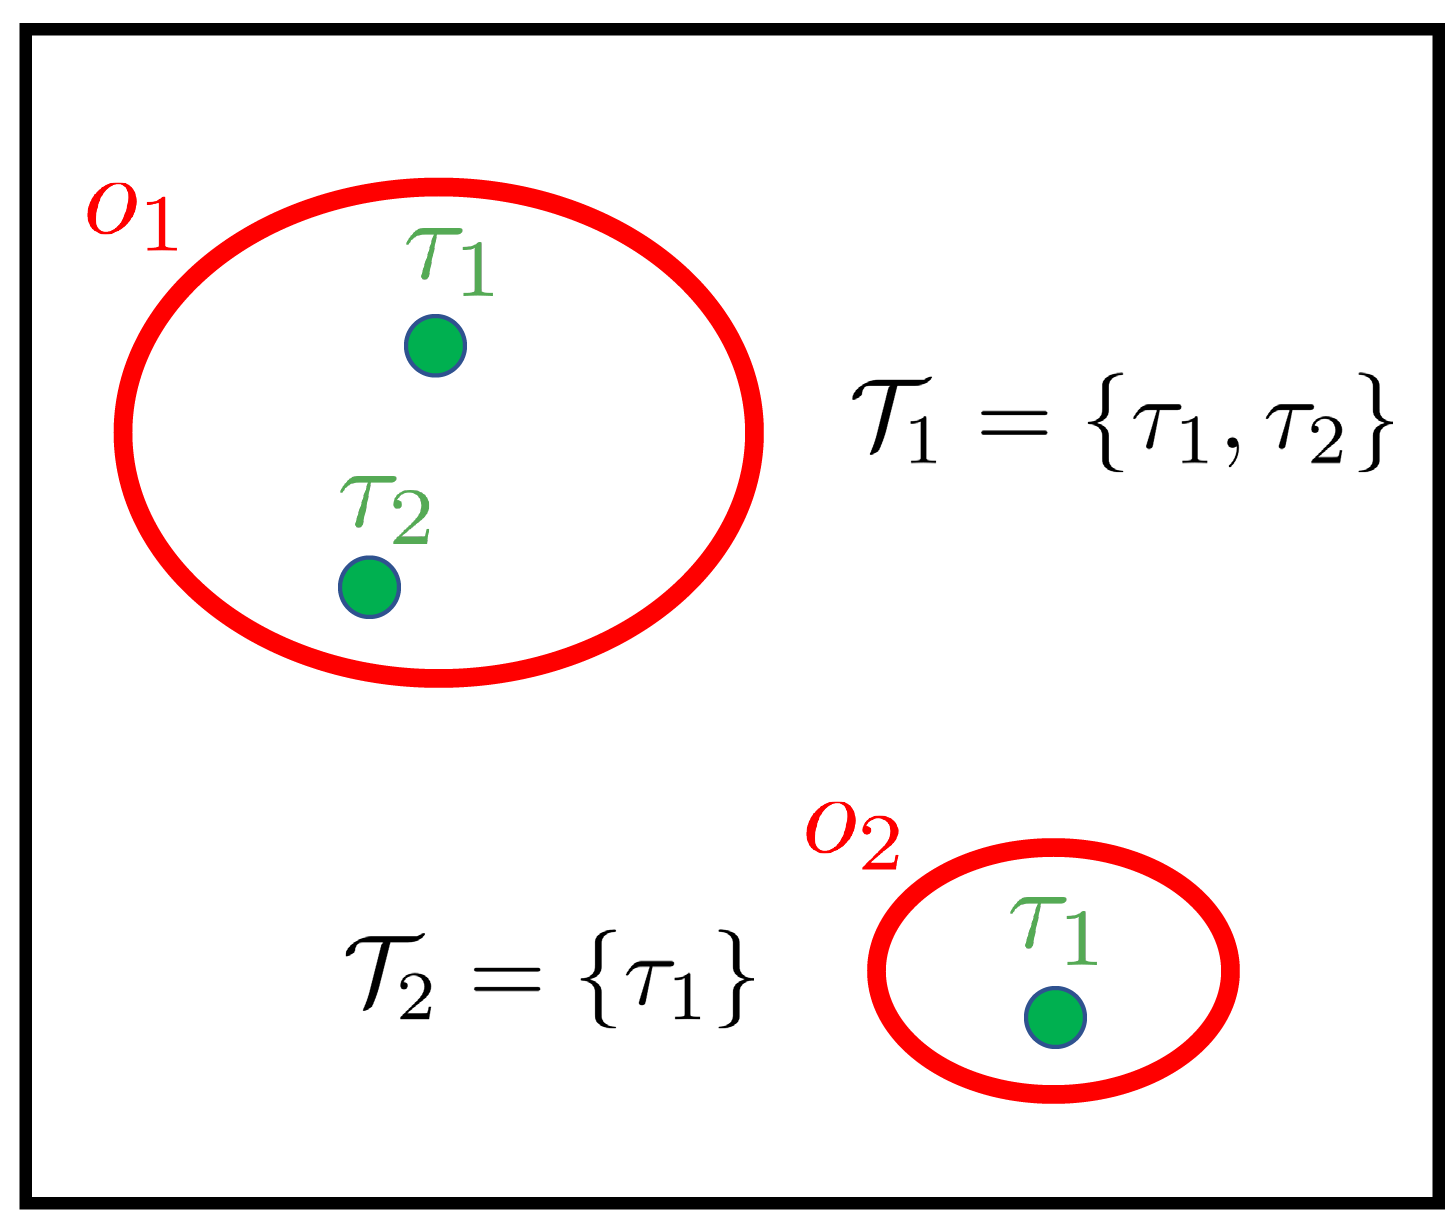
\includegraphics[width=14cm]{fig/TargetSet.png}
% 	\caption{Relationship between targets and tasks. }
% 	\label{fig:TargetSet}
% \end{figure}
% Next, consider $M$ types of heterogeneous robots and the number of robot $m\in\{1,2,...,M\}$ is $N_m\in\mathbb{N}$. 
% The set of robot $m$ can be represented as $\mathcal{R}_m\in\{r^m_1,r^m_2,...,r^m_{N_m}\}$ and the set of robots as a whole as $\mathcal{R}=\mathcal{R}_1\cup ...\cup \mathcal{R}_M$. 
% Each of the $M$ robots perform different tasks, and the set of tasks performed by robot $m$ is $\mathcal{T}_m\subset\mathcal{T}$. 
Next, consider $I$ heterogeneous mobile robots $\mathcal{R}=\{r_1,r_2,...,r_I\}$.
Each type of robot, such as a drone or ground robot, has unique functions and can perform different tasks.
Let consider a set of tasks that can be performed by a robot $i$ with a certain function is $\mathcal{T}_i\subset\mathcal{T}$, and a set of robots that can perform task $j\in\{1,2,...,J\}$ is $\mathcal{R}_j\subset\mathcal{R}$. 
For time, we divide the entire time from the start time to the finish time of all tasks into $L$ steps. 
The set of times is described by $\mathcal{L}=\{1,2,...,L\}$.
For simplicity, this paper assumes that the time step $l\in\mathcal{L}$ is taken so that the robot has enough time to perform the task and to move the target.
Each task for each target be performed at least one period in the entire time, and the set of $k$th performed period set is $\mathcal{L}^k_{hj}\subset\mathcal{L}$. 
Let $l^{ks}_{hj} = \mathrm{arg}\min_{\mathcal{L}^k_{hj}} l$ be the start available time and $l^{kf}_{hj} = \mathrm{arg}\max_{\mathcal{L}^k_{hj}} l$ be the limit time, then all tasks must be performed at time $l$ satisfying $l^{ks}_{hj} \le l \le l^{kf}_{hj}$.
In this paper, we consider allocating robot $i$ at time $l$ satisfying $l^{ks}_{hj} \le l \le l^{kf}_{hj}$ to a target where $\mathcal{J}_{hi}=\mathcal{J}_{i}\cap\mathcal{J}_{h}$, the common set of $\mathcal{J}_h$ and $\mathcal{J}_i$, is $\mathcal{J}_{hi}\neq \varnothing$.

\section{Task and Target Allocation Problem}
In this paper, the problem of assigning tasks to robots and targets is a very complex problem. 
In particular, there are many constraints, such as the different types of tasks that can be executed by each robot and the different tasks that exist for each target, and it is necessary to avoid inappropriate assignments.
Therefore, propositional logic is used to express these constraints. 
Propositional logic can be expressed as a linear inequality using Boolean variables and four arithmetic operations, and can be easily solved as an optimization problem. 
This section describes the linear inequality representation of propositional logic used in this paper and formulates the constraints and specifications for this problem.

\subsection{Inequality Representation of Propositional Logic}
Let $X_p$ denote the logical variable that represents TRUE(T) and FALSE(F) according to [] for proposition $p$. 
The logical operations ``$\vee$~(or)'', ``$\wedge$~(and)'', ``$\bar{\cdot}$~(not)'', ``$\rightarrow$~(imply)'', ``$\leftrightarrow$~(iff)'', and ``$\oplus$~S(exclusive or)'' are introduced into this logical variable. 
The results of these operations are shown in Table \ref{table:Truth Table}.
\begin{table}[hbtp]
    \caption{Truth Table}
    \label{table:Truth Table}
    \centering
    \begin{tabular}{|c|c||c|c|c|c|c|c|}
      \hline
      $X_1$ & $X_2$ & $X_1\vee X_2$ & $X_1\wedge X_2$ & $\bar{X}_1$ & $X_1\rightarrow X_2$ & $X_1\leftrightarrow X_2$ & $X_1\oplus X_2$ \\
      \hline \hline
        F  & F  & F & F & T & T & T & F\\
        F  & T  & T & F & T & T & F & T\\
        T  & F  & T & F & F & F & F & T\\
        T  & T  & T & T & F & T & T & F\\
      \hline
    \end{tabular}
\end{table}

Let introduce an index variable $\delta_p\in\{0,1\}$ and correspond it with $X_p=[\delta_p=1]$.
When then obtain the following corollary.
\begin{corollary}[Inequality Representation of Logical Operations]
    \begin{align}
        &X_1\vee X_2~\mathrm{is~equivalent~to}~\delta_1 + \delta_2 \ge 0\\
        &X_1\wedge X_2~\mathrm{is~equivalent~to}~\delta_1=1,~\delta_2=1\\
        &\sim X_1~\mathrm{is~equivalent~to}~\delta_1 = 0\\
        &X_1\rightarrow X_2~\mathrm{is~equivalent~to}~\delta_1 - \delta_2 \le 0\\
        &X_1\leftrightarrow X_2~\mathrm{is~equivalent~to}~\delta_1 + \delta_2 \le 0\\
        &X_1\oplus X_2~\mathrm{is~equivalent~to}~\delta_1 + \delta_2 = 1
    \end{align}
\end{corollary}
\begin{theorem}
    It is clear from the Table. \ref{table:Truth Table}.
\end{theorem}
Furthermore, the following complement is used to unite propositions in which multiple propositions are joined by $\vee$ or $\wedge$.
\begin{corollary}[Substitution Method]\mbox{}\\
    \begin{itemize}
        \item[(i)] Condition (i)-(a) and (i)-(b) are equivalent.\mbox{}\\
            \begin{itemize}
                \item[(a)]$X_1\leftrightarrow(X_2\vee X_3)$\\
                \item[(b)] $\delta_2-\delta_1\le 0,~\delta_3-\delta_1\le 0,~\delta_2+\delta_3-\delta_1\ge 0$
            \end{itemize}
            \mbox{}\\
        \item[(ii)] Condition (ii)-(a) and (ii)-(b) are equivalent.\mbox{}\\
            \begin{itemize}
                \item[(a)]$X_1\leftrightarrow(X_2\wedge X_3)$\\
                \item[(b)] $\delta_2-\delta_1\ge 0,~\delta_3-\delta_1\ge 0,~\delta_2+\delta_3-\delta_1\le 0$
            \end{itemize}
            \mbox{}\\
    \end{itemize}
\end{corollary}

    
\subsection{Allocation Variables}
To assign robots to tasks and targets, this paper uses an integer programming problem.

The allocation, i.e., the assignment of robots to targets and tasks, is described by a set of Boolen variables $\delta_{ijhl}$ that are set to 1 when the robot $r_i$ performs task $\tau_j$ on target $o_h$ at time $l$ (otherwise it is set to 0).
For convenience, $x$ is defined as the aggregated vector $x=[\delta_{ijhl}]_{i\in\mathcal{R},j\in\mathcal{T},h\in\mathcal{O},l\in\mathcal{L}}$.
% An example of the described variables in time step $l$ can be seen in Fig. ,where tasks and targets have been considered static.







\end{document}
